% pdflatex presentation

\documentclass[svgnames]{beamer}
\usepackage[utf8]{inputenc}
\usepackage[T1]{fontenc}
\usepackage[sfdefault,scaled=.85,lining]{FiraSans}
\usepackage[scaled=0.85,lining]{FiraMono}
\usepackage{newtxsf}
\usepackage{rotating}
\usepackage{listings}
\usepackage{hyperref}

\usetheme{default}
\setbeamertemplate{navigation symbols}
{%
%  \hspace{3em}
%  \vbox{%
%  \hbox{\insertslidenavigationsymbol}
%  \hbox{\insertframenavigationsymbol}
%  \hbox{\insertbackfindforwardnavigationsymbol}
%  \vspace{2em}}
}

\setbeamerfont{frametitle}{family=\sffamily\firamedium}
\setbeamercolor{alerted text}{fg=red!70!black}
\setbeamercolor{structure}{fg=Navy}
\setbeamertemplate{section in toc shaded}[default][30]


\hypersetup{%
  pdftitle={Teaching coding with nbgrader - lessons learned}
  ,pdfauthor={Gert-Ludwig Ingold <gert.ingold@physik.uni-augsburg.de>}
  ,pdfsubject={Talk at Jupyter4edu conference, Katowice 23.9.2019}
  ,pdfkeywords={Python, Jupyterhub, nbgrader, education}
}

\definecolor{positive}{rgb}{0, 0.5, 0}
\definecolor{negative}{rgb}{0.7, 0, 0}
\definecolor{myred}{rgb}{0.8, 0, 0}
\definecolor{mygreen}{rgb}{0, 0.6, 0}
\definecolor{myblue}{rgb}{0, 0, 0.8}

\newcommand\but{\alert{\textit{but}} }

\graphicspath{{./images/}}

\begin{document}

\begin{frame}[t]
 \vspace{1.5truecm}
 \begin{center}
  \structure{\huge\textbf{Teaching coding with nbgrader}}\\[0.2truecm]
  \structure{\huge\textbf{-- lessons learned --}}\\[0.8truecm]
  \structure{\Large Gert-Ludwig Ingold}\\[0.1truecm]
  \structure{\large Universität Augsburg}
 \end{center}
\end{frame}

\begin{frame}{Teaching situation}
 \begin{itemize}
  \item programming language: Python\\
	{\small Dlaczego warto uczyć w języku python? {\scriptsize$\nearrow$} \url{youtu.be/CEmg3gdFlaE}}\\
	{\small Why teach Python? {\scriptsize$\nearrow$} \url{youtu.be/X18jt2lVmJY}}
        \begin{itemize}
	 \item low entry barrier
	 \item expressive code
	 \item well suited for serious work
	 \item freely available, ``batteries included´´
         \item Anaconda distribution for coherent environment on
	       current operating systems
	\end{itemize}
  \item teaching programming to physicists and materials scientists\\
	since 2010, typically 10+ students
  \item next year: mandatory course for 100+ students
 \end{itemize}

\end{frame}

\begin{frame}{Coping with heterogeneity}
 \begin{itemize}
  \item students without programming experience and (sometimes) code writing apprehension
  \item students with knowledge in another programming language\\
	code often does not look very pythonic\\
	example: loop over objects vs. loop over indices
 \end{itemize}

 students with programming experience should not be bored and should obtain an interesting
 result from their code

 \begin{itemize}
  \item \but scientific applications are often considered as an extra mental burden
 \end{itemize}
\end{frame}

\begin{frame}{nbgrader}
 \begin{itemize}
  \item tool that facilitates creating and grading assignments in the Jupyter notebook
  \item distributing and collecting assignments
  \item automatic grading by means of unit tests
  \item manual grading possible
  \item feedback can be given to students
 \end{itemize}

 \begin{itemize}
  \item freely available
  \item open source
  \item latest version: 0.6.0 released end of August 2019
 \end{itemize}
\end{frame}

\begin{frame}{nbgrader on Github}
 \begin{center}
  \url{github.com/jupyter/nbgrader/}

  \vspace{0.3truecm}
  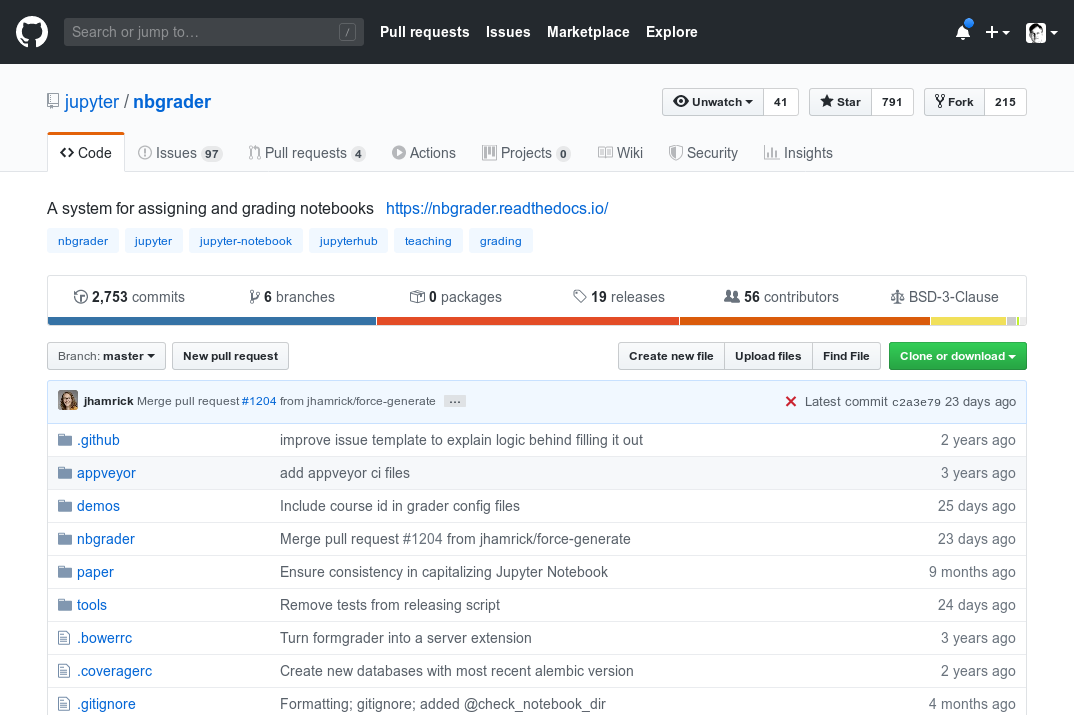
\includegraphics[width=\textwidth]{nbgrader_github}
 \end{center}
\end{frame}

\begin{frame}{Github issues for nbgrader}
 \begin{center}
  report and discuss problems or new features

  \vspace{0.3truecm}
  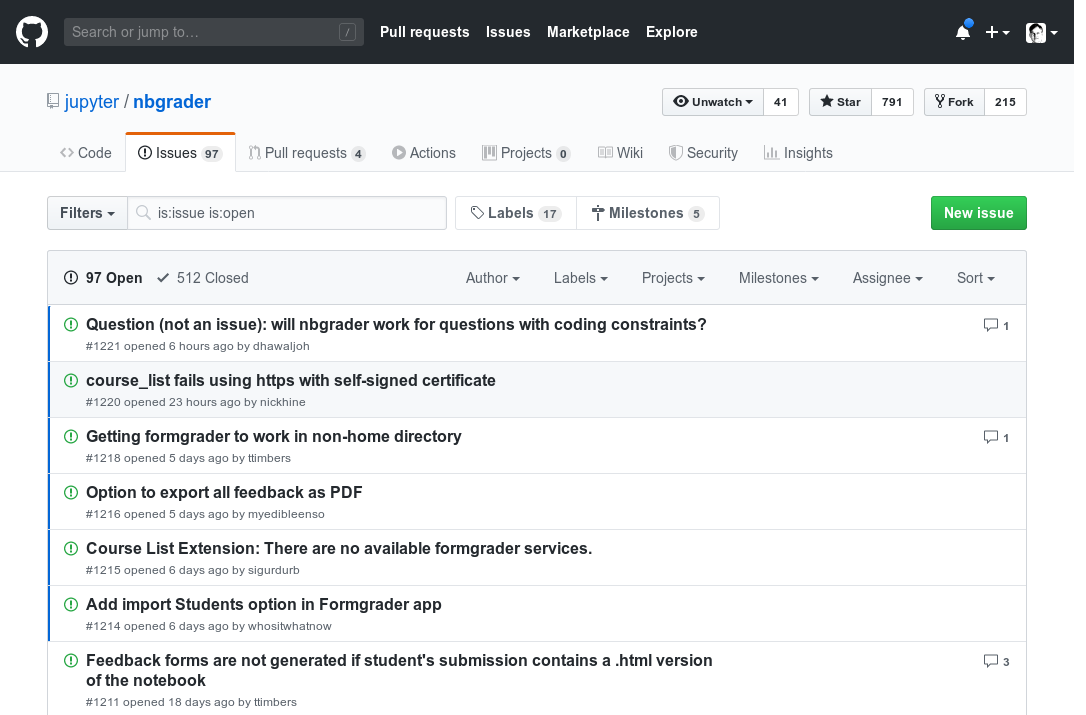
\includegraphics[width=\textwidth]{nbgrader_githubissues}
 \end{center}
\end{frame}

\begin{frame}{Pull requests for nbgrader}
 \begin{center}
  contribute to the code or the documentation

  \vspace{0.3truecm}
  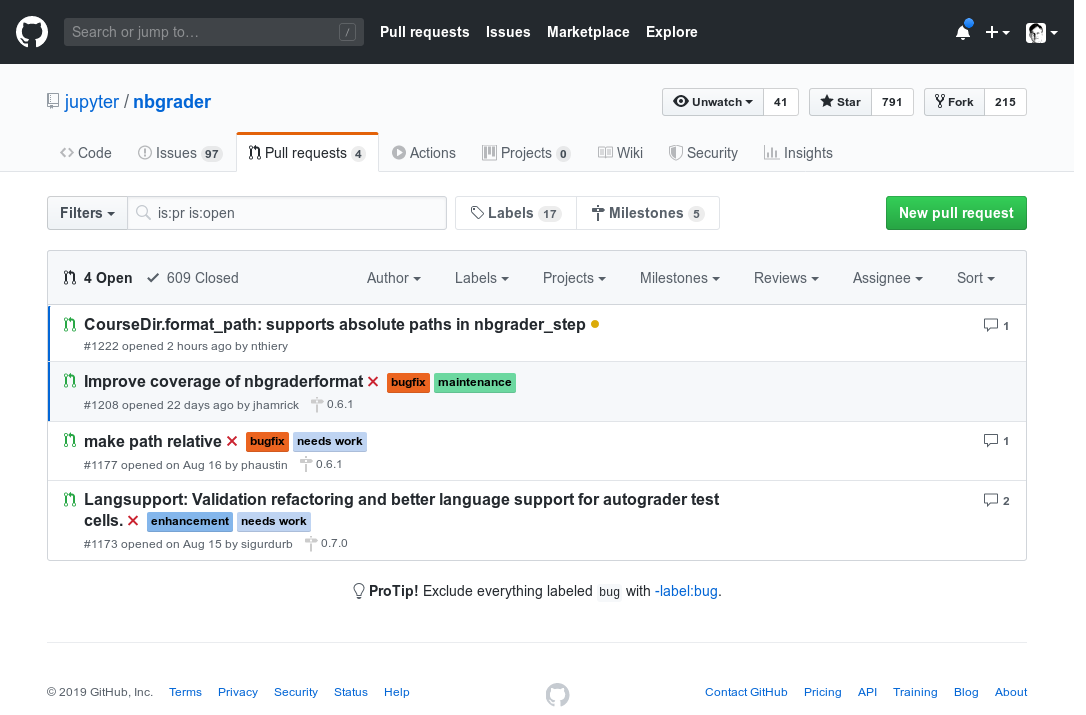
\includegraphics[width=\textwidth]{nbgrader_githubprs}
 \end{center}
\end{frame}

\begin{frame}{nbgrader documentation}
 \begin{center}
  \url{nbgrader.readthedocs.io}

  \vspace{0.3truecm}
  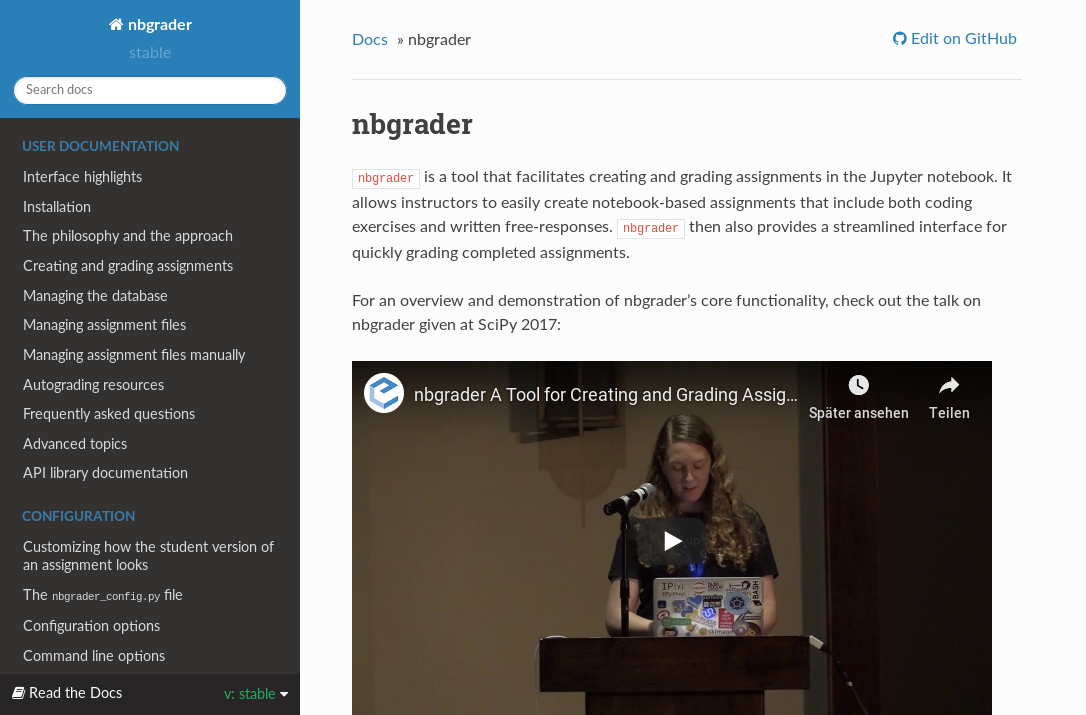
\includegraphics[width=\textwidth]{nbgrader_rtd}
 \end{center}
\end{frame}

\begin{frame}{Jupyter notebook and Jupyterhub -- pros and cons}

 \structure{Jupyter notebook}
 \begin{itemize}
  \item notebook allows to guide students through a problem set
  \item problems related to out-of-order execution
  \item students might think that programming in Python
	necessarily implies working with a Jupyter notebook,
        they should know about IDEs (spyder, \dots) and
	editors (vim, \dots)
 \end{itemize}

 \structure{Jupyterhub}
 \begin{itemize}
  \item easily accessible interface to problem sets
  \item no need to install Python on local computer
  \item consistent working environment for all students
  \item \but may be beginners should gather experience with Python
	on their own computer
 \end{itemize}
\end{frame}

\begin{frame}{Functions}
 \begin{center}
  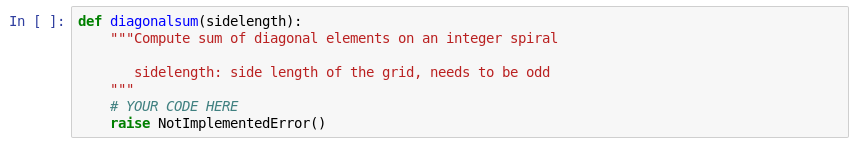
\includegraphics[width=\textwidth]{examplecell}
 \end{center}

 \vspace{0.3truecm}
 \begin{itemize}
  \item need to introduce functions very early in the course\\
	\but special aspects (no arguments, no return value, default arguments,
	keyword arguments, \dots) not needed
  \item students get used to logically structured code early on\\
	\but they do not do it themselves
  \item include docstrings to make task well defined\\
	students get used to the idea that a function contains a docstring\\
        \but they are not writing the docstring by themselves
 \end{itemize}
\end{frame}

\begin{frame}{Grading with tests}
 \begin{center}
  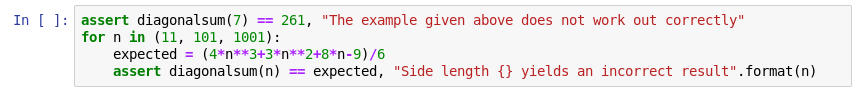
\includegraphics[width=\textwidth]{tests}
 \end{center}

 \vspace{0.3truecm}
 \begin{itemize}
  \item test-driven development\\
	\but tests are not developed by the students
  \item tests allow to give feedback through error messages\\
	\but students tend to rely on this feedback instead of developing their
	own critical view on their code
  \item ``Stupid mistakes'' will be made not only at the beginning
	\begin{itemize}
         \item ``trivial'' standard tests (are results returned, do they have the correct type, \dots?)
	 \item + tests of specific functionality which should not disclose the solution
	\end{itemize}
 \end{itemize}
 \begin{center}
  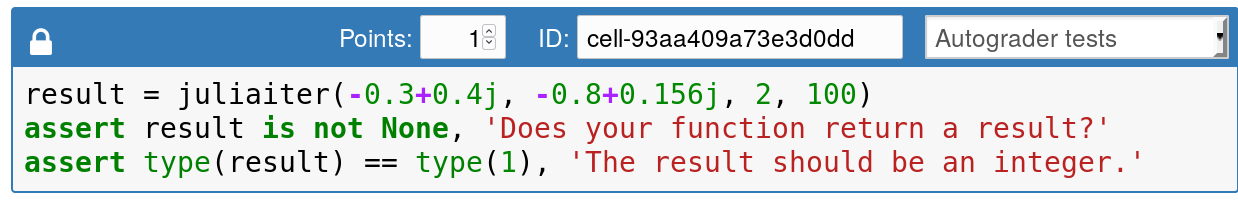
\includegraphics[width=\textwidth]{answer_tests_unittest1}
 \end{center}
\end{frame}

\begin{frame}{Examples of problem sets I}

 \vspace{-0.7truecm}
 \begin{columns}[t]
  \begin{column}{0.5\textwidth}
   \begin{center}
    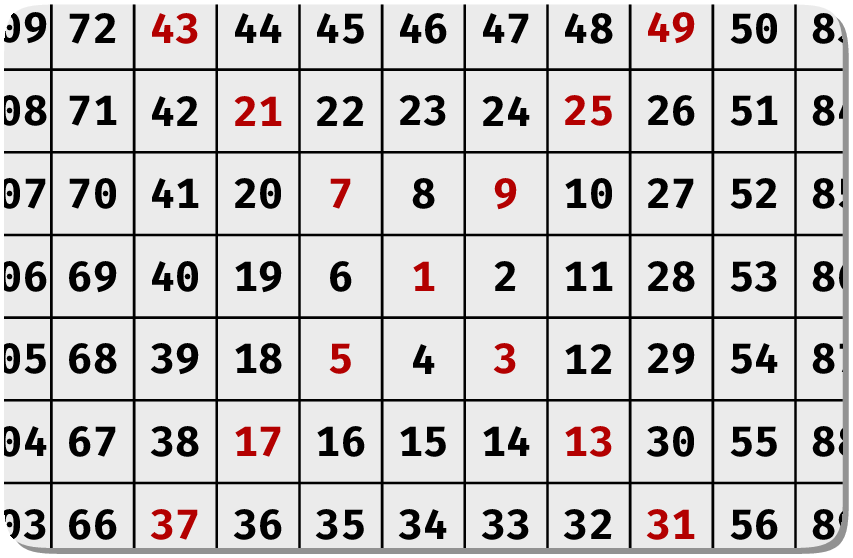
\includegraphics[width=0.8\textwidth]{spiral}

    a problem from\\[-0.05truecm] Project Euler (\url{projecteuler.net})
   \end{center}
  \end{column}%
  \begin{column}{0.5\textwidth}
   \begin{center}
    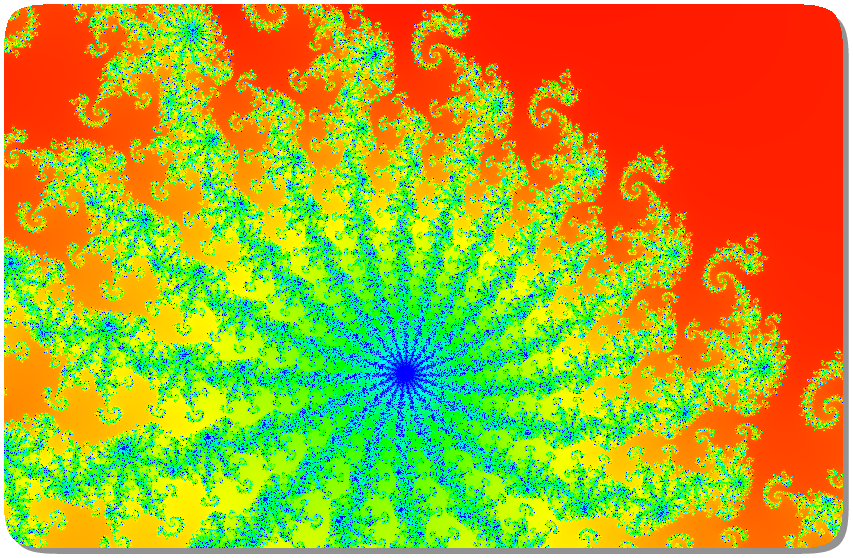
\includegraphics[width=0.8\textwidth]{julia}

    Julia set
   \end{center}
  \end{column}%
 \end{columns}

 \begin{columns}[t]
  \begin{column}{0.5\textwidth}
   \begin{center}
    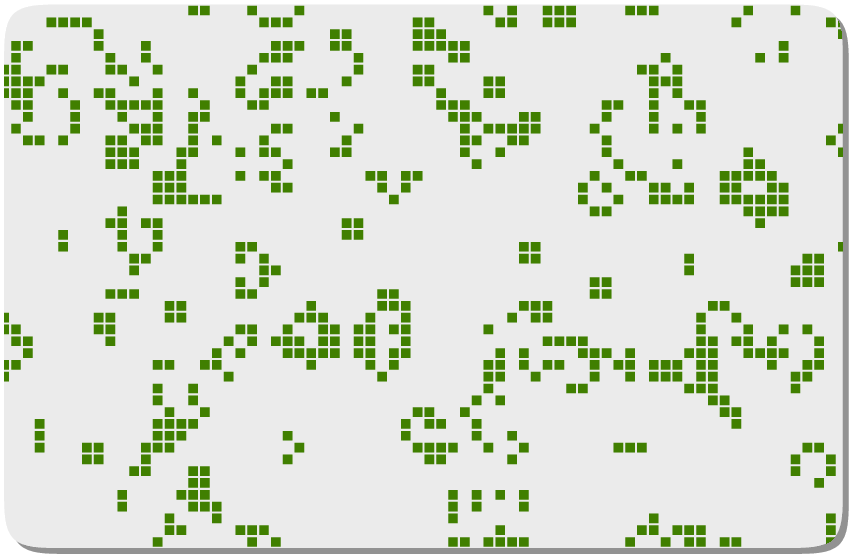
\includegraphics[width=0.8\textwidth]{conway}

    Conway's game of life
   \end{center}
  \end{column}%
  \begin{column}{0.5\textwidth}
   \begin{center}
    
\includegraphics[width=0.8\textwidth]{pi}

    $\pi$ to a few thousand digits
   \end{center}
  \end{column}%
 \end{columns}

 \vspace{0.4truecm}
 {\scriptsize\url{https://github.com/marcinofulus/jupyter4edu/tree/master/augsburg/exercises}}
\end{frame}

\begin{frame}{Examples of problem sets II}

 \vspace{-0.7truecm}
 \begin{columns}[t]
  \begin{column}{0.5\textwidth}
   \begin{center}
    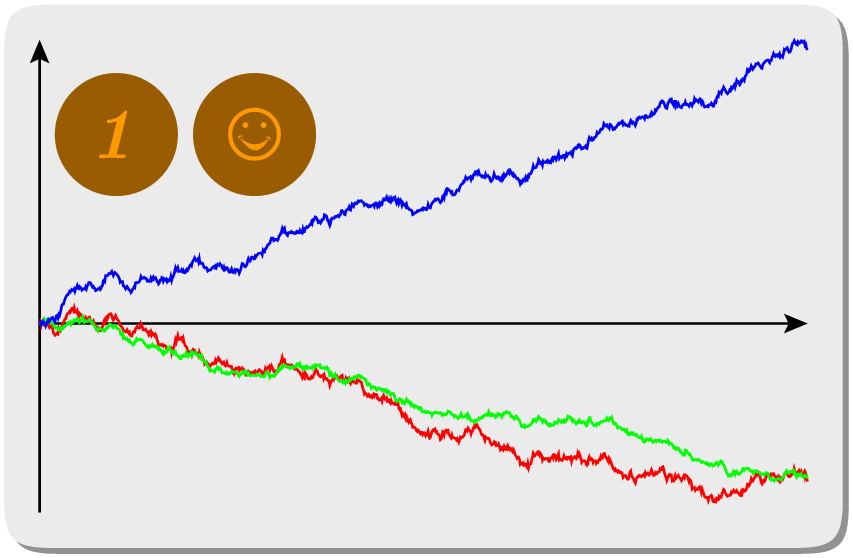
\includegraphics[width=0.8\textwidth]{parrondo}

    Parrondo paradoxon
   \end{center}
  \end{column}%
  \begin{column}{0.5\textwidth}
   \begin{center}
    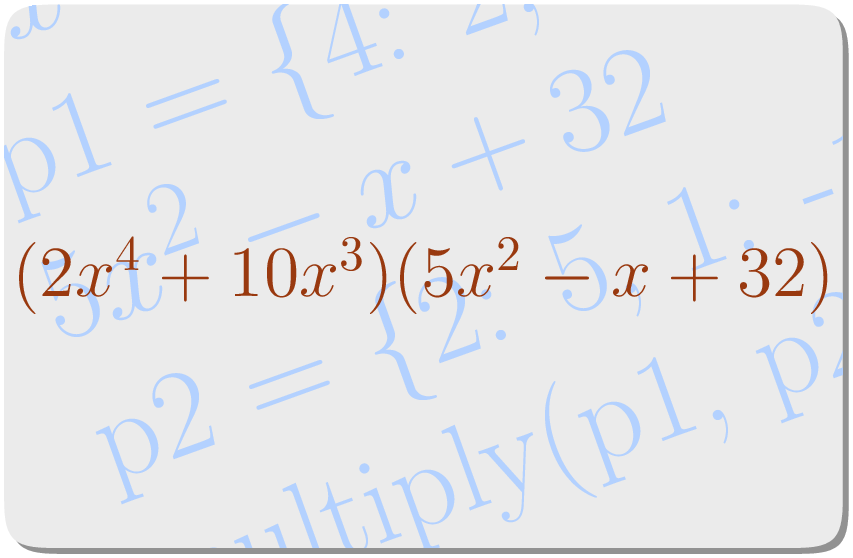
\includegraphics[width=0.8\textwidth]{polynomial}

    symbolic manipulation of polynomials
   \end{center}
  \end{column}%
 \end{columns}

 \begin{columns}[t]
  \begin{column}{0.5\textwidth}
   \begin{center}
    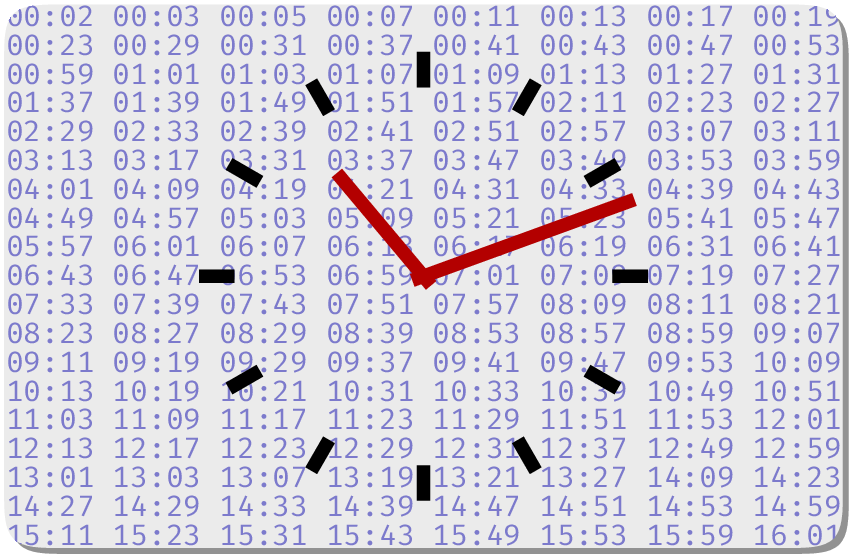
\includegraphics[width=0.8\textwidth]{primetime}

    How many primes are times?
   \end{center}
  \end{column}%
  \begin{column}{0.5\textwidth}
   \begin{center}
    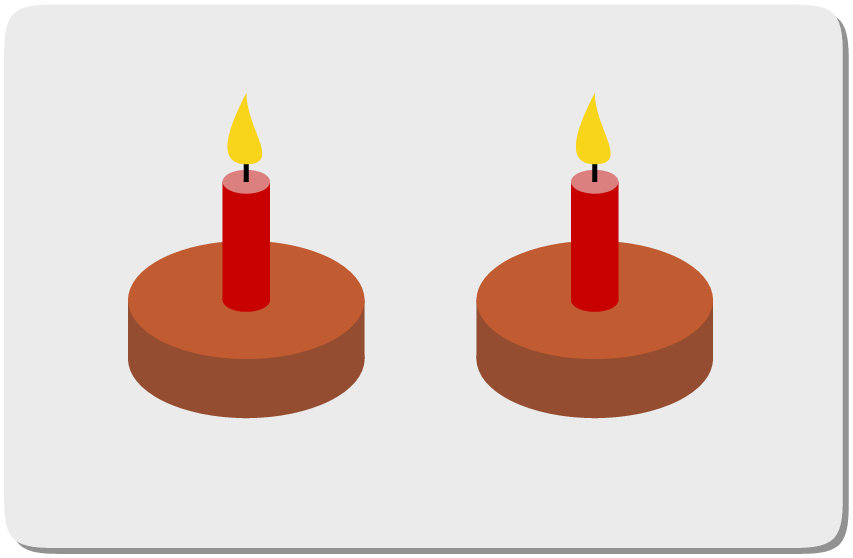
\includegraphics[width=0.8\textwidth]{birthday}

    birthday problem
   \end{center}
  \end{column}%
 \end{columns}

 \vspace{0.4truecm}
 {\scriptsize\url{https://github.com/marcinofulus/jupyter4edu/tree/master/augsburg/exercises}}
\end{frame}

\begin{frame}{Branching paths}
 \only<1>{%
  \begin{columns}
   \begin{column}{0.3\textwidth}
    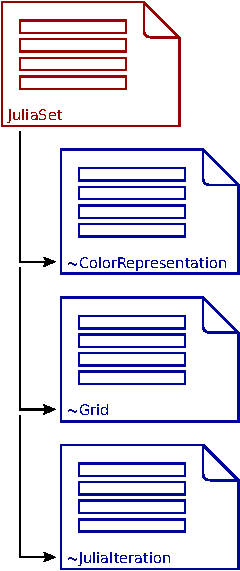
\includegraphics[height=0.8\textheight]{branching_1}
   \end{column}%
   \begin{column}{0.7\textwidth}
    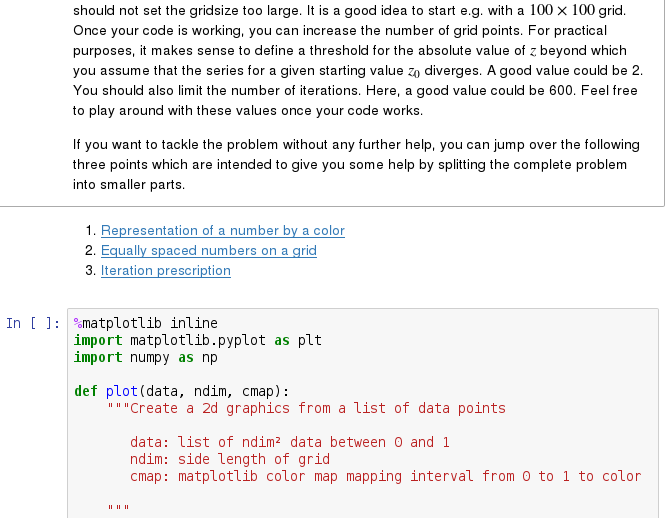
\includegraphics[width=\textwidth]{JuliaSet_screenshot}
   \end{column}
  \end{columns}
 }%
 \only<2>{%
  \begin{columns}
   \begin{column}{0.3\textwidth}
    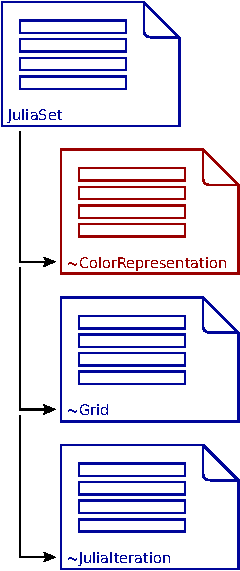
\includegraphics[height=0.8\textheight]{branching_2}
   \end{column}%
   \begin{column}{0.7\textwidth}
    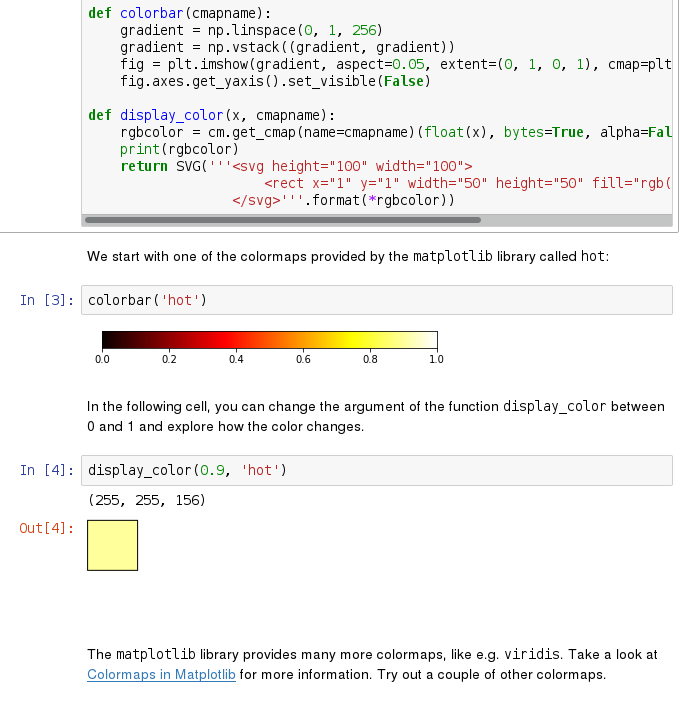
\includegraphics[width=\textwidth]{ColorRepresentation_screenshot}
   \end{column}
  \end{columns}
 }%
 \only<3>{%
  \begin{columns}
   \begin{column}{0.3\textwidth}
    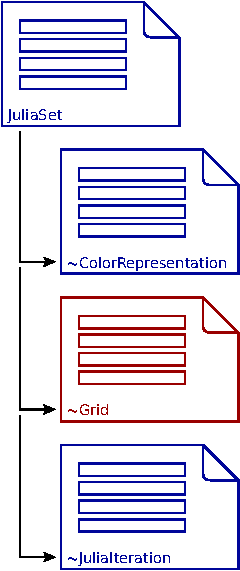
\includegraphics[height=0.8\textheight]{branching_3}
   \end{column}%
   \begin{column}{0.7\textwidth}
    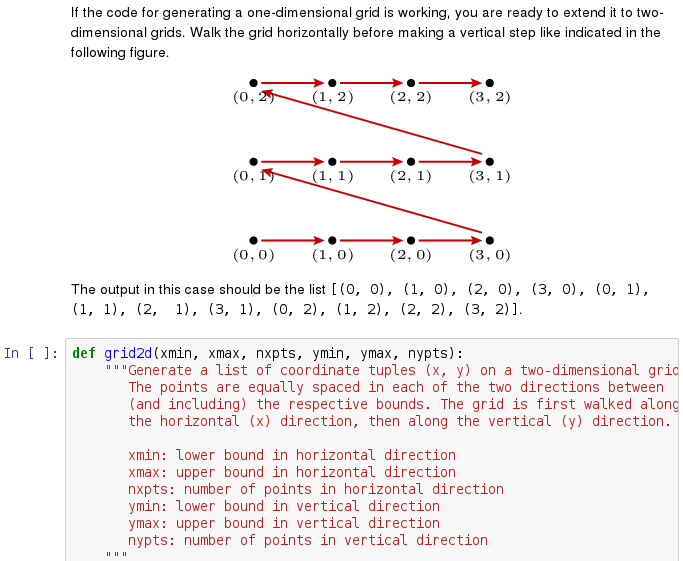
\includegraphics[width=\textwidth]{Grid_screenshot}
   \end{column}
  \end{columns}
 }%
 \only<4>{%
  \begin{columns}
   \begin{column}{0.3\textwidth}
    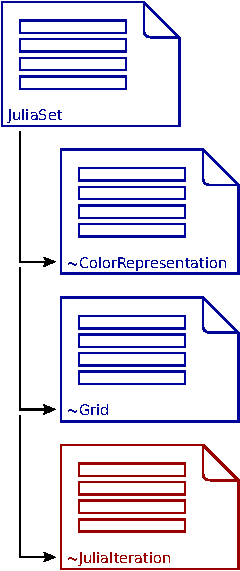
\includegraphics[height=0.8\textheight]{branching_4}
   \end{column}%
   \begin{column}{0.7\textwidth}
    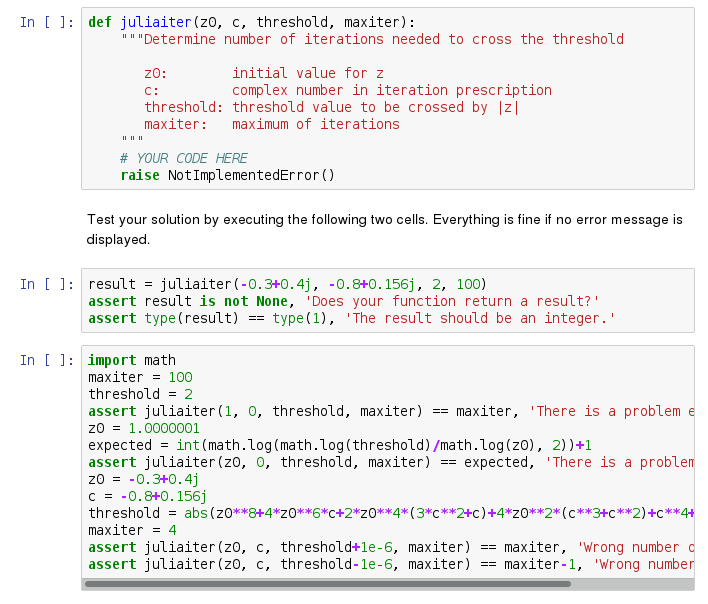
\includegraphics[width=\textwidth]{JuliaIteration_screenshot}
   \end{column}
  \end{columns}
 }%
 \only<5>{%
  \begin{columns}[b]
   \begin{column}{0.3\textwidth}
    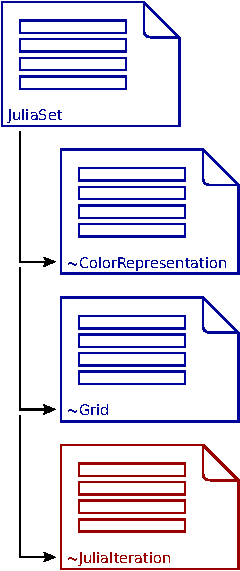
\includegraphics[height=0.8\textheight]{branching_4}
   \end{column}%
   \begin{column}{0.7\textwidth}
    \begin{itemize}
     \item individual path through problem possible
     \item \but notebooks are opened in new tabs, it is easy to lose track
    \end{itemize}

    \vspace{1truecm}
   \end{column}
  \end{columns}
 }
\end{frame}

\end{document}
